\documentclass[12pt,a4paper,bibliography=totocnumbered,listof=totocnumbered]{scrartcl}
\usepackage[utf8]{inputenc}
\usepackage{amsmath}
\usepackage{amsfonts}
\usepackage{amssymb}
\usepackage{graphicx}
\usepackage{fancyhdr}
\usepackage{tabularx}
\usepackage{geometry}
\usepackage{setspace}
\usepackage[right]{eurosym}
\usepackage[printonlyused]{acronym}
\usepackage{subfig}
\usepackage{floatflt}
\usepackage[usenames,dvipsnames]{color}
\usepackage{colortbl}
\usepackage{paralist}
\usepackage{array}
\usepackage{titlesec}
\usepackage{parskip}
\usepackage[right]{eurosym}
\usepackage{colortbl}
\usepackage[subfigure,titles]{tocloft}
\usepackage[pdfpagelabels=true]{hyperref}
\usepackage[round]{natbib}
\usepackage{listings}


\lstset{basicstyle=\footnotesize, captionpos=b, breaklines=true, showstringspaces=false, tabsize=2, frame=lines, numbers=left, numberstyle=\tiny, xleftmargin=2em, framexleftmargin=2em, language=python}
\makeatletter
\def\l@lstlisting#1#2{\@dottedtocline{1}{0em}{1em}{\hspace{1,5em} Lst. #1}{#2}}
\makeatother

\geometry{a4paper, top=27mm, left=30mm, right=20mm, bottom=35mm, headsep=10mm, footskip=12mm}

\hypersetup{unicode=false, pdftoolbar=true, pdfmenubar=true, pdffitwindow=false, pdfstartview={FitH},
	pdftitle={Bachelorarbeit},
	pdfauthor={Alina Asisof},
	pdfsubject={Bachelorarbeit},
	pdfcreator={\LaTeX\ with package \flqq hyperref\frqq},
	pdfproducer={pdfTeX \the\pdftexversion.\pdftexrevision},
	pdfkeywords={Bachelorarbeit},
	pdfnewwindow=true,}

\pdfinfo{/CreationDate (D:20110620133321)}


\begin{document}

\titlespacing{\section}{0pt}{12pt plus 4pt minus 2pt}{-6pt plus 2pt minus 2pt}

% Kopf- und Fusszeile
\renewcommand{\sectionmark}[1]{\markright{#1}}
\renewcommand{\leftmark}{\rightmark}
\pagestyle{fancy}
\lhead{ }
\chead{ }
\rhead{\thesection\space\contentsname}
\lfoot{Software Engineering}
\cfoot{ }
\rfoot{\ \linebreak Seite \thepage}
\renewcommand{\headrulewidth}{0.4pt}
\renewcommand{\footrulewidth}{0.4pt}

% Vorspann
\renewcommand{\thesection}{\Roman{section}}
\renewcommand{\theHsection}{\Roman{section}}
\pagenumbering{Roman}

% ----------------------------------------------------------------------------------------------------------
% Titelseite
% ----------------------------------------------------------------------------------------------------------
\thispagestyle{empty}
\begin{center}
	
	\vspace*{2cm}
	\Huge
	\textbf{Software Engineering}\\
\vfill
	\Large
	\textbf{The effect of the abandonment of the Swiss Franc - Euro parity on tourism}\\
\vfill
	\Large
	{Prof. Dr. Philipp Zahn}\\
	\Large
	University of St. Gallen
	
\vfill


\end{center}

\begin{flushleft}	
	\vfill
	\normalsize
\textbf{Submitted by:} \\
Alina Asisof, Master of Business Innovation HSG\\
Student Number: 12-749-677\\ 
Carla Walker, Master of Business Innovation HSG\\ 
Student Number: 12-611-091\\ 

Joao Matias, Bachelor of Economics University of Lissabon\\ 
Student Number: 16-601-809\\ 
\vfill
Group Project Documentation\\ 
 
\vfill
\textbf{18. January 2017}

\end{flushleft}	



\pagebreak

% ----------------------------------------------------------------------------------------------------------
% Verzeichnisse
% ----------------------------------------------------------------------------------------------------------
% TODO Typ vor Nummer

\renewcommand{\cftfigpresnum}{Abb. }
\settowidth{\cfttabnumwidth}{Abb. 10\quad}
\settowidth{\cftfignumwidth}{Abb. 10\quad}

\titlespacing{\section}{0pt}{12pt plus 4pt minus 2pt}{2pt plus 2pt minus 2pt}
\singlespacing
\rhead{CONTENT}
\renewcommand{\contentsname}{Content}

\phantomsection
\addcontentsline{toc}{section}{\texorpdfstring{\hspace{0.35em}Content}{Content}}
\addtocounter{section}{1}
\tableofcontents
\pagebreak

%\pagebreak


\pagebreak


% ----------------------------------------------------------------------------------------------------------
% Inhalt
% ----------------------------------------------------------------------------------------------------------
% Abstände Überschrift
\titlespacing{\section}{0pt}{12pt plus 4pt minus 2pt}{-6pt plus 2pt minus 2pt}
\titlespacing{\subsection}{0pt}{12pt plus 4pt minus 2pt}{-6pt plus 2pt minus 2pt}
\titlespacing{\subsubsection}{0pt}{12pt plus 4pt minus 2pt}{-6pt plus 2pt minus 2pt}

% Kopfzeile
\renewcommand{\sectionmark}[1]{\markright{#1}}
\renewcommand{\subsectionmark}[1]{ }
\renewcommand{\subsubsectionmark}[1]{ }
\lhead{Chapter \thesection}
\rhead{\rightmark}

\onehalfspacing
\renewcommand{\thesection}{\arabic{section}}
\renewcommand{\theHsection}{\arabic{section}}
\setcounter{section}{0}
\pagenumbering{arabic}
\setcounter{page}{1}

%--------------------
%Einleitung
%--------------------

\section{Introduction}

%What problem does our project solve ? 
%For what will our code be used? 
%Research question: What effect had the abandonment of the Swiss Franc - Euro parity of January 2015 on tourism within and outside of Switzerland? 
%How does the strong CHF influence travel behavior? 
%CHF goes up - people travel more outside of Switzerland? 
%How will we analyze this? 
%What are the tools that we are going to use? Python and Latex. 


On January 15th the Swiss National Bank decided to abandon the Swiss Franc - Euro parity of 1.20:1. The financial markets reacted immediately: The exchange rate fell drastically and a Euro temporarily was worth less than 0.8 Swiss Francs. The decision surprised experts and executives alike and evoked great concerns regarding the future competitiveness of the Swiss industries. Some of the analysis are yet to be made and conclusions to be drawn. The risen value of the Swiss currency also left the national tourism industry sorrowful, as hotel owners and owners of popular touristic attractions alike feared a diminishing number of foreign tourists and hence missing out on revenue. Our project will focus on the tourism industry: We will conduct a simple regression to see, whether the decision of the Swiss National Bank on abandoning the parity had any effect on the national tourism industry. Did the tourism in the country decline or did it remain unchanged? How did the strong Swiss Franc influence the travel behavior within and outside of Switzerland? Are the Swiss traveling more since January 15th due to the risen value of their currency? Can we conclude an impact on tourism on the basis of tourist numbers? 

We will analyze this by using a data set provided by the Federal Statistical Office. The Federal Statistical Office publishes a variety of data on tourism throughout the year. For 2015 there is a comprehensive set of data available, gathered in form of Excel-files and officially published. For the year 2016 there is a data set available gathering the data of the first half of the year which we will use as a proxy for the year 2016, since more recent data will not be available before February. These data sets will be compared to the data before January 15th/2015 and a regression on the exchange rate of the Swiss Franc to Euro will be made. We will therefore use financial data published at "Finanzen.net", so both sources are trustworthy and well known. We will compute a regression with the help of a code written in Python on Spyder. To do that, we will remotely collaborate with the help of GitHub, a platform used to write code in groups. GitHub will also help us with the coordination and collaboration challenge connected to our project.\\
For the documentation of our project we have used LateX, as it is a tool easily embedding both Python Code and different types of content. \\
\\
We will first introduce our data set and parameters. In the following chapter we will conduct the regression and present the results of our Python code. We will add a short explanation on the code, so that the code can be easily understood and reproduced. In the last part we will conclude on the tourism effects of the parity abandonment and assess, to what extend the concerns expressed by hotel owners and experts were justified. 


\newpage


% ----------------------------------------------------------------------------------------------------------
% 
% ----------------------------------------------------------------------------------------------------------
\section{Dataset}



Our term paper researches the question how the abandonment of the Swiss franc - Euro parity influences Swiss tourism. To analyze the question, we compared two datasets. The first one is the historical exchange rate between the Euro and the Swiss franc. The second dataset is from the Federal Statistical Office on the chronological development of travels with overnight stays of the Swiss population from 15 years old (Swiss Federal Statistical Office, 2016). 


As the Swiss Exchange Rate to the Euro was falling for several years, the Swiss National Bank of Switzerland decided on September 6, 2011 to fix the minimum exchange rate of 1.20 Franc for one Euro. The SNB declared, that the minimum exchange rate will be enforced with all the consequences and that it is willing to buy unlimited foreign exchanges (SNB, 2011). With this action step, the Swiss National Bank reacted to the constant threat of the Swiss Economy and the risk of a deflationary trend which resulted from the massive overvaluation of the Swiss Franc. On January 15, the Swiss National Bank discontinued the minimum exchange rate of 1.20 Franc to the Euro (SNB, 2015). The Swiss National Bank declared that maintaining the minimum exchange rate for the Swiss franc against the Euro is no longer justified. The Swiss Economy which is oriented towards export and tourism, reacted with great concernes. 

\begin{figure}[htbp] 
  \centering
     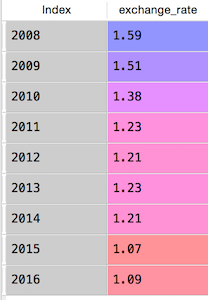
\includegraphics[width=0.3\textwidth]{exchange_variable}
  \caption{Variable explorer in Python}
  \label{fig: figure1}
\end{figure}

For our term paper, we took data from Statista, a statistics portal. The statistic chosen displays the annual exchange rate (standardized measure) of the Euro to the Swiss franc (EUR-CHF), according to the data of the European Central Bank. We only considered the data from the years 2008 to 2016. In 2008, for example, the Euro to Swiss franc exchange rate was equal to approximately 1.59, which means that one euro could buy 1.59 Swiss francs. In 2015, the Euro to Swiss franc exchange rate was equal to approximately 1.07, which means that one euro could only buy 1.07 Swiss francs (Statista, 2016). This resulted in huge value losses of European valuta and made the Swiss Franc savings more valuable.


The Federal Statistical Office provides a detailed dataset of the chronological development of travels with overnight stays. This dataset contains statistical information regarding the private domestic tourism expenses and private tourism expenses of the Swiss Nationals abroad per person and day. This information includes accomodation expenses as well as money spent on meals and drinks, transportation costs and other costs. The dataset also includes information on the amount of foreign travels (travels outside of Switzerland) and travels within the boundaries of the Swiss territory in thousand. We can therefore compare, wheter either of the parameters changes with regard to the other when plotted against the exchange rate. The dataset is available as an Excel-table for download. The table also contains information such as the number of travels per person, the demographics of the people who travelled and more detailed information about the travels itself, including the duration, the purpose, the type of accommodation, the means of transport, the destination and more. This information is not considered in this paper.

For our research, we decided on the following parameters: expenses - domestic and abroad, number of travels - in Switzerland and abroad. The goal is that further parameters can be analyzed in relationship with the exchange rate through our code very easily. 

%Here comes something on Data Management. Maybe a short explanation of what we did with the excel files? 


\newpage
\section{Linear Regression}
A Linear regression assumes a linear relation between the input variables (X) and the single output variable (Y). We assume a linear change in the expenses people are willing to make abroad and "at home" with respect to the value of the valuta. We also expect a linear relation between the exchange rate as a relative value of one currency to the other and the number of travels. A low exchange rate, e.g. 1.07 CHF/Euro means, that travelling abroad becomes comparably cheaper and travelling domestically becomes relatively more expensive. We hence expect a positive linear relation between exchange rates and domestic travels and a negative linear relation between exchange rates and travels abroad. Whe expect similar relations between the exchange rate and domestic expenses resp. expenses abroad: A rising exchange rate hinders people of spending money abroad whereas a sinking exchange rate should theoretically foster the spending of money abroad.\\ We tested this theoretical approach by executing a linear regression via Python. \\
\subsection{Data Management}
In order to execute a regression written in Python we first had to set up a file to manage the data. We parsed multiple Exel-Files in order to combine the data. The output will be a table with a column for the data in each exel file, which each row corresponding to a given year. Concretely, the parameters described above will appear in a single merged file in columns indexed by year. 
\subsection{Reading the Data}

To do this we first had to import some software libraries such as \textit{pandas} which is providing us with easy to use data structures and data analysis. We also imported the \textit{glob} module since we use a wildcard pattern to import our data. 

In the end we set the directory of the data import files and used the module \textit{glob} to create a list with all the Research variables files in the data folder:

\begin{verbatim}
import pandas as pd
import glob
# set directory of data import files
# @var curr = files directory
curr = "../softwareengineering/Data/RV*.xlsx"
glob.glob(curr)
\end{verbatim}


Afterwards we created the Data Frame. This is neccesary to append all the different rows with our data according to the same year in columns:
\begin{verbatim}
dataset = pd.DataFrame()
for f in glob.glob(curr):
df =p d.read_excel(f)
dataset = dataset.append(df, ignore_index=True)
dataset = dataset.set_index("year").T
\textit{# bug fixing}
dataset = dataset.reset_index().rename(columns={"index" : "year"})
dataset.columns.name = None
dataset.set_index("year", inplace = True)
\end{verbatim}

With this we can now print the transposed data set and receive a table:

\begin{figure}[htbp] 
  \centering
     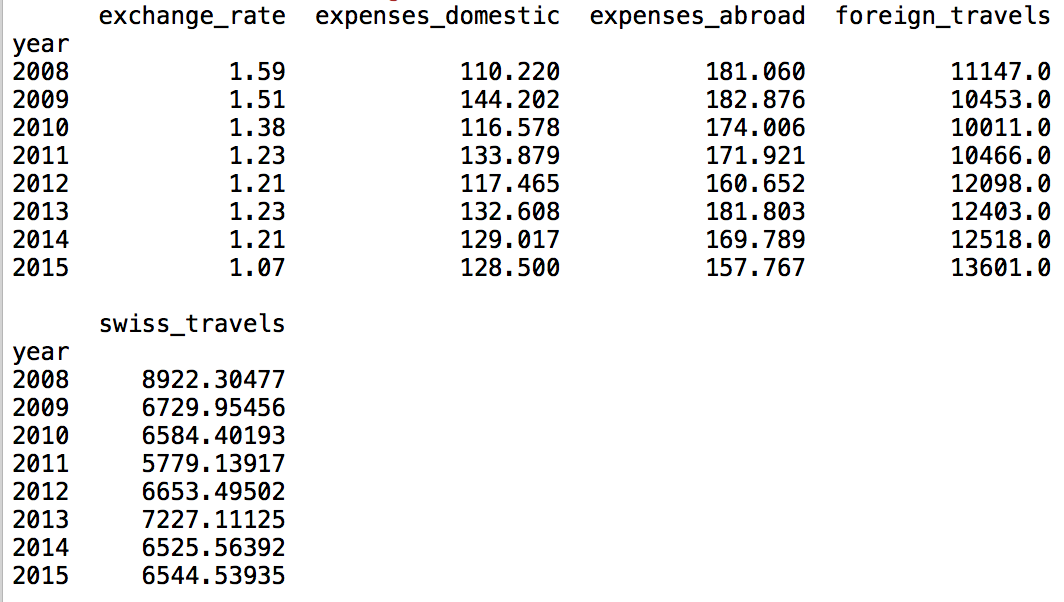
\includegraphics[width=0.3\textwidth]{data_table}
  \caption{data set according to parameters and year }
  \label{fig: figure2}
\end{figure}



\subsection{Plotting}
With \textit{sklearn} which is a machine learning library allowing for regression and mean computations and interoperating with another scientific library called \textit{NumPy} we can now execute high-level mathematical functions like coefficients. With \textit{matplotlib} which is a plotting library, we can then plot the results after importing the dataset. 

\begin{verbatim}
from sklearn import linear_model
import matplotlib.pylot as plt
import numpy as np
\textit{import dataset from the Datamanagement Module}
from datamanagement import dataset
\end{verbatim}

Now we are ready to plot the variables against each other. We defined, that x_df is the dataframe column for the exchange rate, whereas the y_df is the dataframe column for the y-value, which can be exchanged for any of the four parameters chosen. 
\begin{verbatim}
x_df = dataset.loc[:,["exchange_rate"]]
y_df = dataset.loc[:,["swiss_travels"]]
\end{verbatim}


Now we can run the regression, plot the results and ask our interface to return the graphs:
\begin{verbatim}
regr = linear_model.LinearRegression()
regr.fit(x_df, y_df)
\textit{plot outputs and show the graph}
plt.scatter(x_df, y_df, color='black')
plt.plot(x_df, regr.predict(x_df), color='blue', linewidth=3)
plt.show()
\end{verbatim}

The plotted graph for the Swiss travels in dependence of the exchange rate is displayed as follows: 
\begin{figure}[htbp] 
  \centering
     \includegraphics[width=0.3\textwidth]{regression_number_of_Swiss_travels}
  \caption{Regression of number of Swiss travels}
  \label{fig: figure3}
\end{figure}
We can now see the relation between the variables for every single column just by changing the \textit{y}-Variable. We can hence recreate the regression with any of the four parameters we have already described in the dataset chapter. 

\subsection{Coefficients}
In a last step we conduct the coefficients, the mean sqare error and the variance:
\begin{verbatim}
print('Coefficients: \n', regr.coef_)
print("Mean squared error: \%.2f" \% np.mean((regr.predict(x_df) - y_df) ** 2))
print('Variance score: \%.2f' \% regr.score(x_df, y_df))
\end{verbatim}

%\subsection{something}
\newpage
\section{Conclusion}

We have plotted the four columns of our data set and concluded the following results: 

%Here comes something 



\section{Team and work progress summary}
The team consisted of three members. The team members had already some experience with basic LaTex, but little or no experience with Python and also never worked with GitHub before. After some start difficulties and a lot of trial and error, the team started to get along with the tools. Especially video tutorials online helped to navigate and operate on GitHub. In order to avoid version clashes we coordinated our working time with the help of social media, since we quickly learned that it is otherwise neccesary to approve/disregard all the changes that happened on the document in the meantime. To program a working linear regression needed more time and more research. The large amount of help material available online for many problems that occurred and suggestions to embellish the code were implemented, where the solutions worked. The code was written partially in Switzerland, where two team members had the opportunity to meet physically and amended and improved remotely by the third member. Once the code was set and we got some routine in working with LaTex we examined the result of the data regression and wrote a conclusion. Working with Python on a regular basis is necessary. Only with some routine the programming language becomes beneficial and easy to use. Our team had a steep learning curve when writing the paper and understood, that a large part of the work is invisible, namely finding bugs when pieces of code are no longer running or lead to intuitively wrong results, trying out solutions and failing forward and doing research on better and more universal ways of coding. Nevertheless our team considered this experience very valuable for our technology-led future working place and we will further enhance the knowledge we have gotten throughout the working progress with this paper.

%
%----------------------------------------------------------------------------------------------------------

% ----------------------------------------------------------------------------------------------------------


%\section{blabla} ----------------------------------------------------------------------------------------------------------

% ----------------------------------------------------------------------------------------------------------
% Literatur
% ----------------------------------------------------------------------------------------------------------

% Literaturliste soll im Inhaltsverzeichnis auftauchen
Swiss Federal Statistical Office. 2016. "Zeitliche Entwicklung der Reisen mit Übernachtungen, Wohnbevölkerung ab 15 Jahren". From: https://www.bfs.admin.ch/bfs/de/home/statistiken/tourismus.assetdetail.1585234.html, retrieved 15.12.2016

%\bibliographystyle{eehd_url}


% Literaturliste endgültig anzeigen
%\bibliography{literatur}

%-------------------


% ----------------------------------------------------------------------------------------------------------
% Anhang
% ----------------------------------------------------------------------------------------------------------

\section{Appendix}



\subsection{Tables}

\subsection{Statistics}





\end{document}




